% Options for packages loaded elsewhere
\PassOptionsToPackage{unicode}{hyperref}
\PassOptionsToPackage{hyphens}{url}
%
\documentclass[
  10pt,
  ignorenonframetext,
]{beamer}
\usepackage{pgfpages}
\setbeamertemplate{caption}[numbered]
\setbeamertemplate{caption label separator}{: }
\setbeamercolor{caption name}{fg=normal text.fg}
\beamertemplatenavigationsymbolsempty
% Prevent slide breaks in the middle of a paragraph
\widowpenalties 1 10000
\raggedbottom
\setbeamertemplate{part page}{
  \centering
  \begin{beamercolorbox}[sep=16pt,center]{part title}
    \usebeamerfont{part title}\insertpart\par
  \end{beamercolorbox}
}
\setbeamertemplate{section page}{
  \centering
  \begin{beamercolorbox}[sep=12pt,center]{section title}
    \usebeamerfont{section title}\insertsection\par
  \end{beamercolorbox}
}
\setbeamertemplate{subsection page}{
  \centering
  \begin{beamercolorbox}[sep=8pt,center]{subsection title}
    \usebeamerfont{subsection title}\insertsubsection\par
  \end{beamercolorbox}
}
\AtBeginPart{
  \frame{\partpage}
}
\AtBeginSection{
  \ifbibliography
  \else
    \frame{\sectionpage}
  \fi
}
\AtBeginSubsection{
  \frame{\subsectionpage}
}
\usepackage{amsmath,amssymb}
\usepackage{iftex}
\ifPDFTeX
  \usepackage[T1]{fontenc}
  \usepackage[utf8]{inputenc}
  \usepackage{textcomp} % provide euro and other symbols
\else % if luatex or xetex
  \usepackage{unicode-math} % this also loads fontspec
  \defaultfontfeatures{Scale=MatchLowercase}
  \defaultfontfeatures[\rmfamily]{Ligatures=TeX,Scale=1}
\fi
\usepackage{lmodern}
\ifPDFTeX\else
  % xetex/luatex font selection
\fi
% Use upquote if available, for straight quotes in verbatim environments
\IfFileExists{upquote.sty}{\usepackage{upquote}}{}
\IfFileExists{microtype.sty}{% use microtype if available
  \usepackage[]{microtype}
  \UseMicrotypeSet[protrusion]{basicmath} % disable protrusion for tt fonts
}{}
\makeatletter
\@ifundefined{KOMAClassName}{% if non-KOMA class
  \IfFileExists{parskip.sty}{%
    \usepackage{parskip}
  }{% else
    \setlength{\parindent}{0pt}
    \setlength{\parskip}{6pt plus 2pt minus 1pt}}
}{% if KOMA class
  \KOMAoptions{parskip=half}}
\makeatother
\usepackage{xcolor}
\newif\ifbibliography
\setlength{\emergencystretch}{3em} % prevent overfull lines
\providecommand{\tightlist}{%
  \setlength{\itemsep}{0pt}\setlength{\parskip}{0pt}}
\setcounter{secnumdepth}{-\maxdimen} % remove section numbering
\usepackage{booktabs}

\usepackage{color, colortbl}
\definecolor{Gray}{gray}{0.9}

\def\begincols{\begin{columns}}
\def\begincol{\begin{column}}
\def\endcol{\end{column}}
\def\endcols{\end{columns}}

\setbeamertemplate{caption}[numbered]
\setbeamertemplate{itemize items}[default]
\setbeamertemplate{itemize subitem}[circle]

\usepackage{ctex} % CJK 包
%\setCJKmainfont[AutoFakeBold = {2.25}]{宋体}
%\usepackage[UTF8]{ctex}

\logo{
\includegraphics[scale=0.2]{bbk200}}
%\usetheme{Madrid}
%\usefonttheme{serif}

%\pgfdeclareimage[scale=0.2]{logo}{bbk2}
%\logo{\pgfuseimage{logo}}

% \begincols
% \begincol{.48\textwidth}
% \endcol
% \begincol{.48\textwidth}
% \endcol
% \endcols

% How many criminal candidates were there? Where and when?
% 6,499 out of 35,075 contesting candidates -- close to 20\%

% Did criminal candidates win elections? Where and when?
% Given that a candidate is a criminal, the probability of winning the election is about 0.22; in contrast, Given that a candidate is NOT a criminal, the probability of winning the election is about 0.12. (X)

% How many criminal politicians were there? Where and when? 

% Party affiliations: BJP (23\%), Congress (18\%), 
\usepackage{bookmark}
\IfFileExists{xurl.sty}{\usepackage{xurl}}{} % add URL line breaks if available
\urlstyle{same}
\hypersetup{
  hidelinks,
  pdfcreator={LaTeX via pandoc}}

\title{\hfill\break
\hfill\break
CP\(^2\) Week 2: From Empire to Nation-State\\
\strut \\}
\author{Dr Chao-Yo Cheng\\}
\date{}

\begin{document}
\frame{\titlepage}

\begin{frame}{Recap: Studying Chinese politics in the changing world}
\phantomsection\label{recap-studying-chinese-politics-in-the-changing-world}
\begin{itemize}
  \item From intelligence services to academic research
  \vspace{0.5cm}
  \item From area studies to comparative politics
  \vspace{0.5cm}
  \item From qualitative description to data-intensive inference
\end{itemize}
\end{frame}

\begin{frame}
\begin{itemize}
  \item From intelligence services to new geopolitcal tension
  \vspace{0.1cm}
  \begin{itemize}
    \item China studies $\neq$ Sinology; emerging as a subject area after the WWII and gain its prominence during the Cold War
    \item "Echo chambers" in the making -- the changing geopolitical landscape in the past decade may drag China scholars in different countries to focus on different agenda
  \end{itemize}
  \vspace{0.3cm}
  \item From area studies to comparative politics
  \vspace{0.3cm}
  \item From qualitative description to data-intensive inference
\end{itemize}
\end{frame}

\begin{frame}
\begin{center}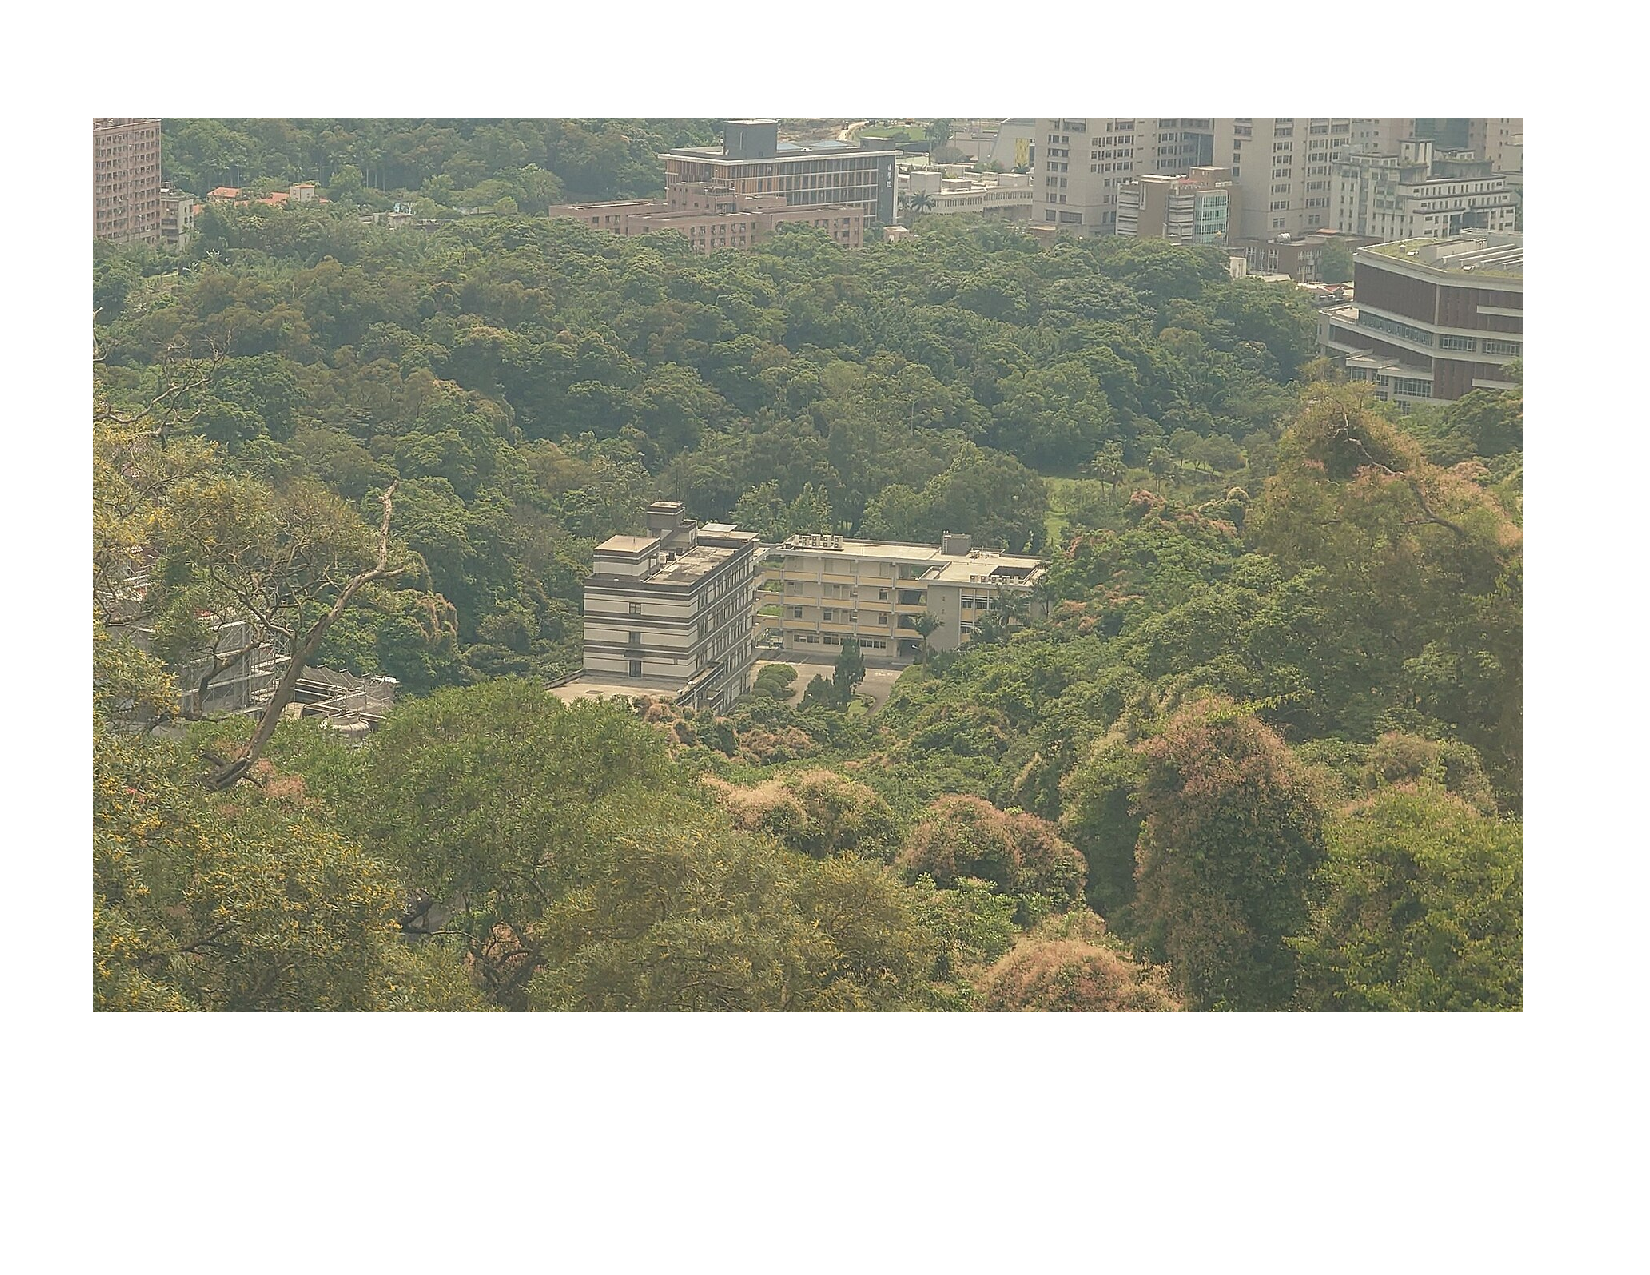
\includegraphics[width=0.8\linewidth]{Figs/nccu} \end{center}
\vspace{0.3cm}
\begin{center}
\small
Institute of International Relations, National Chengchi University (Taipei)
\end{center}
\end{frame}

\begin{frame}
\begin{itemize}
  \item From intelligence services to academic research
  \vspace{0.3cm}
  \item From area studies to comparative politics
  \vspace{0.1cm}
  \begin{itemize}
    \item Earlier generations of China scholars treat China as a distinct subfield within political science
    \item Later on, China scholars begin to borrow or "stretch" concepts and ideas from other subfields to study Chinese politics (Shambaugh 2023)
    \item Starting from the late 2000s, China scholars are about to generate new theoretical insights to general political science (Tsai 2017)
  \end{itemize}
  \vspace{0.3cm}
  \item From qualitative description to data-intensive inference
\end{itemize}
\end{frame}

\begin{frame}
\begin{center}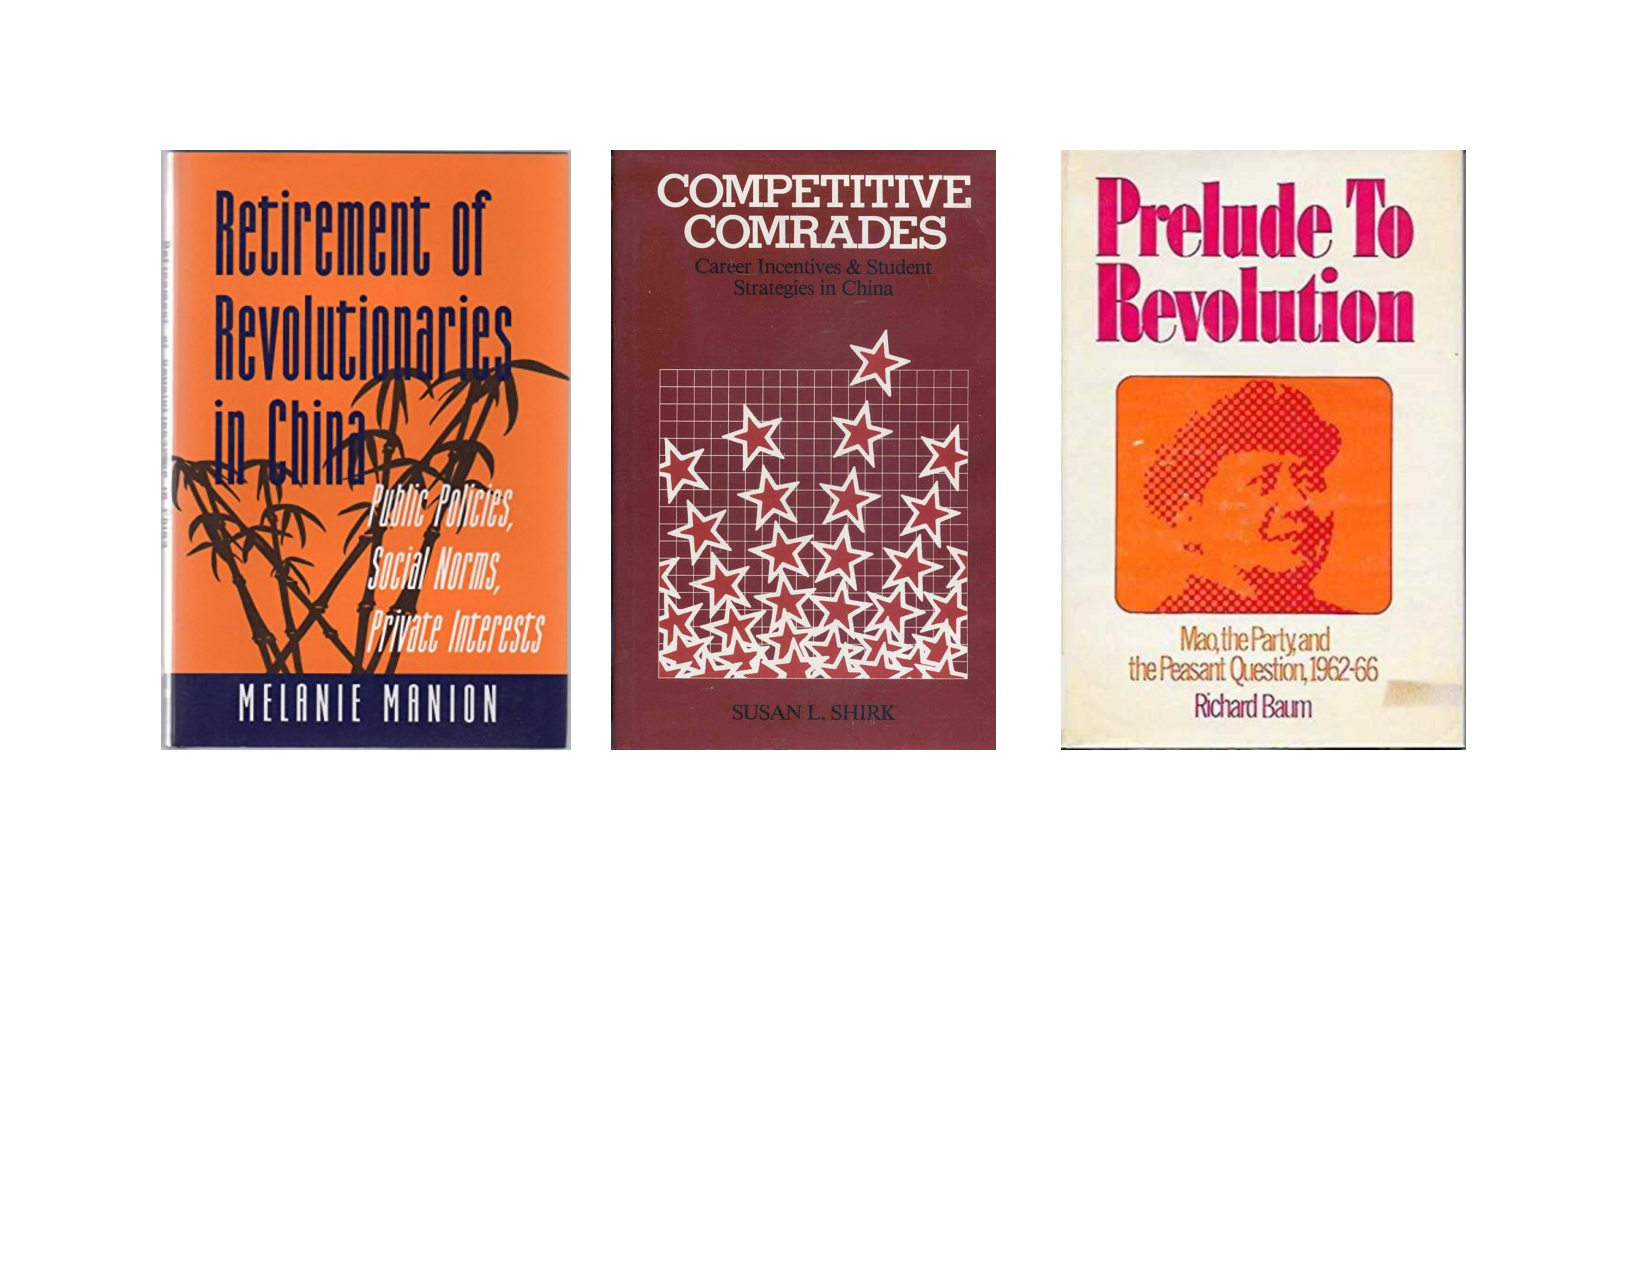
\includegraphics[width=1\linewidth]{Figs/book1} \end{center}
\end{frame}

\begin{frame}
\begin{center}\includegraphics[width=1\linewidth]{Figs/book2} \end{center}
\end{frame}

\begin{frame}
\begin{center}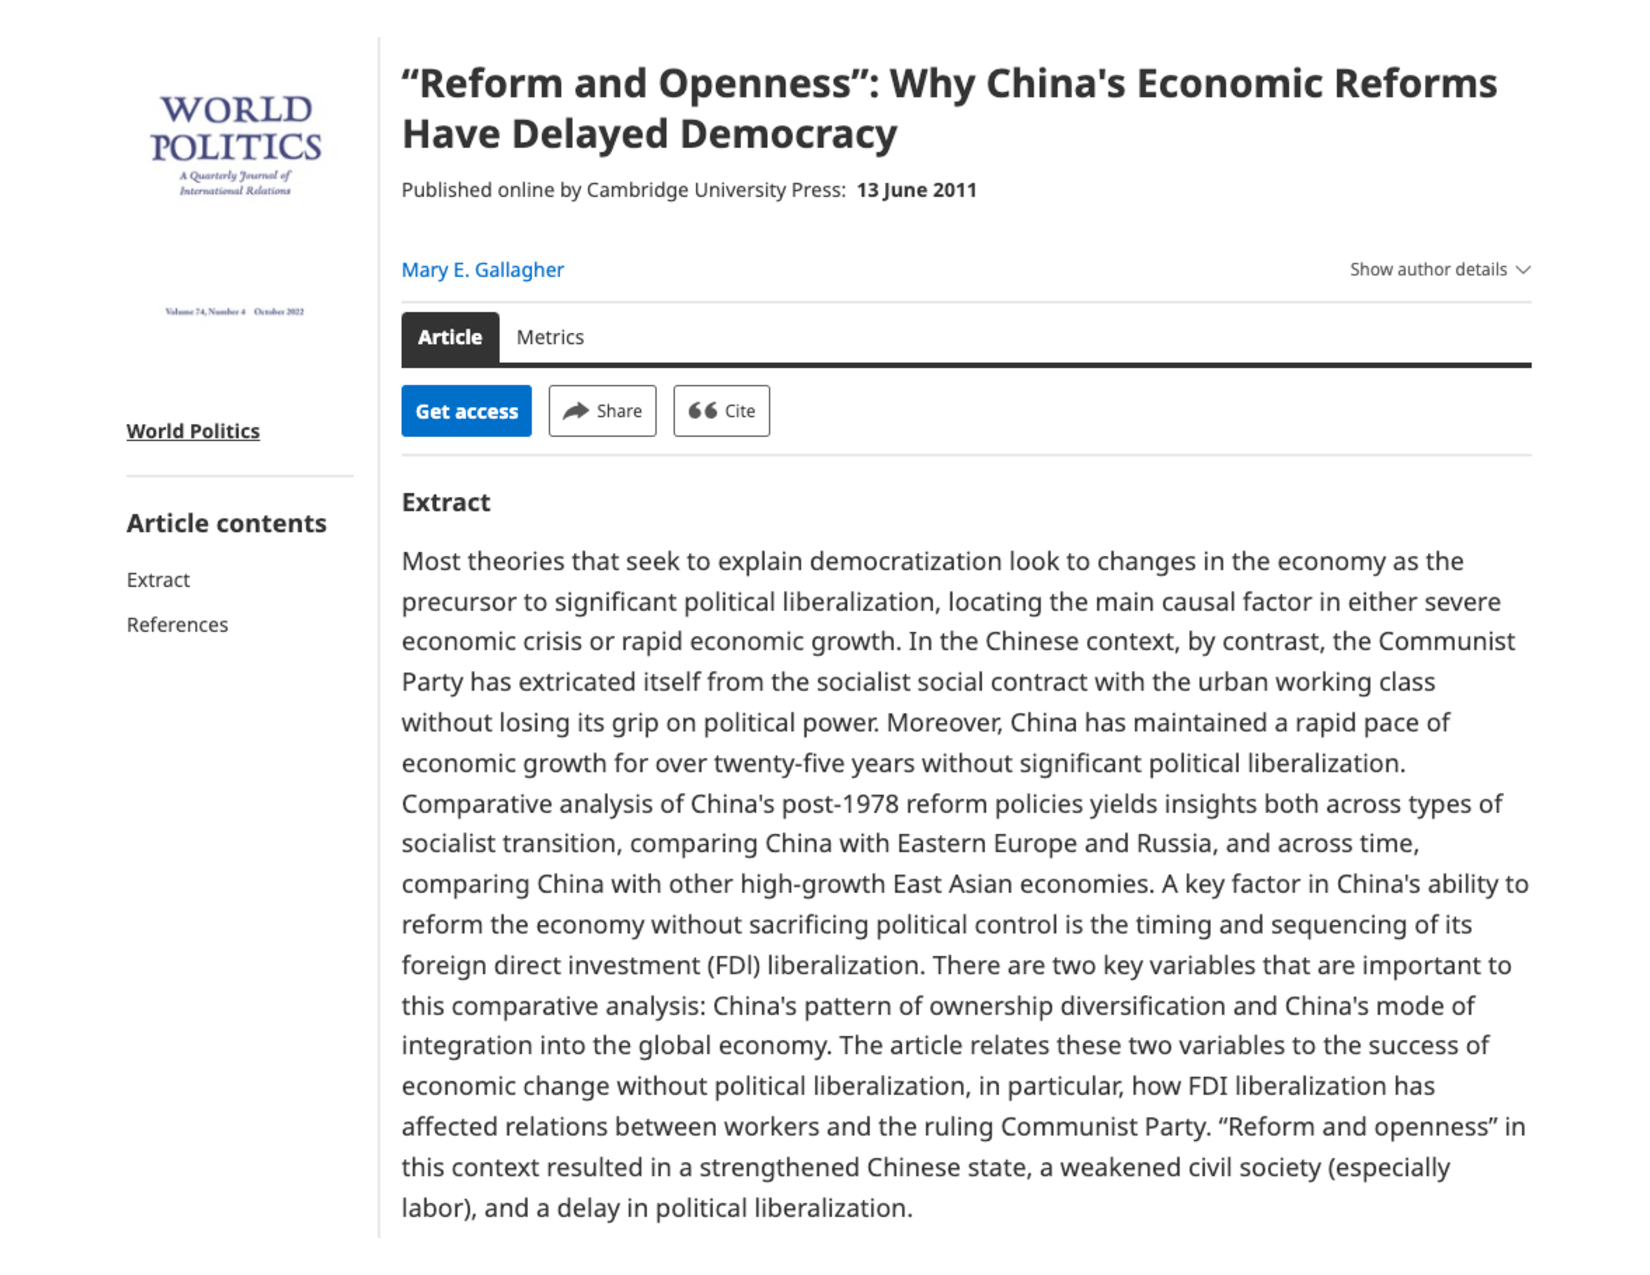
\includegraphics[width=1\linewidth]{Figs/mary} \end{center}
\end{frame}

\begin{frame}
\begin{center}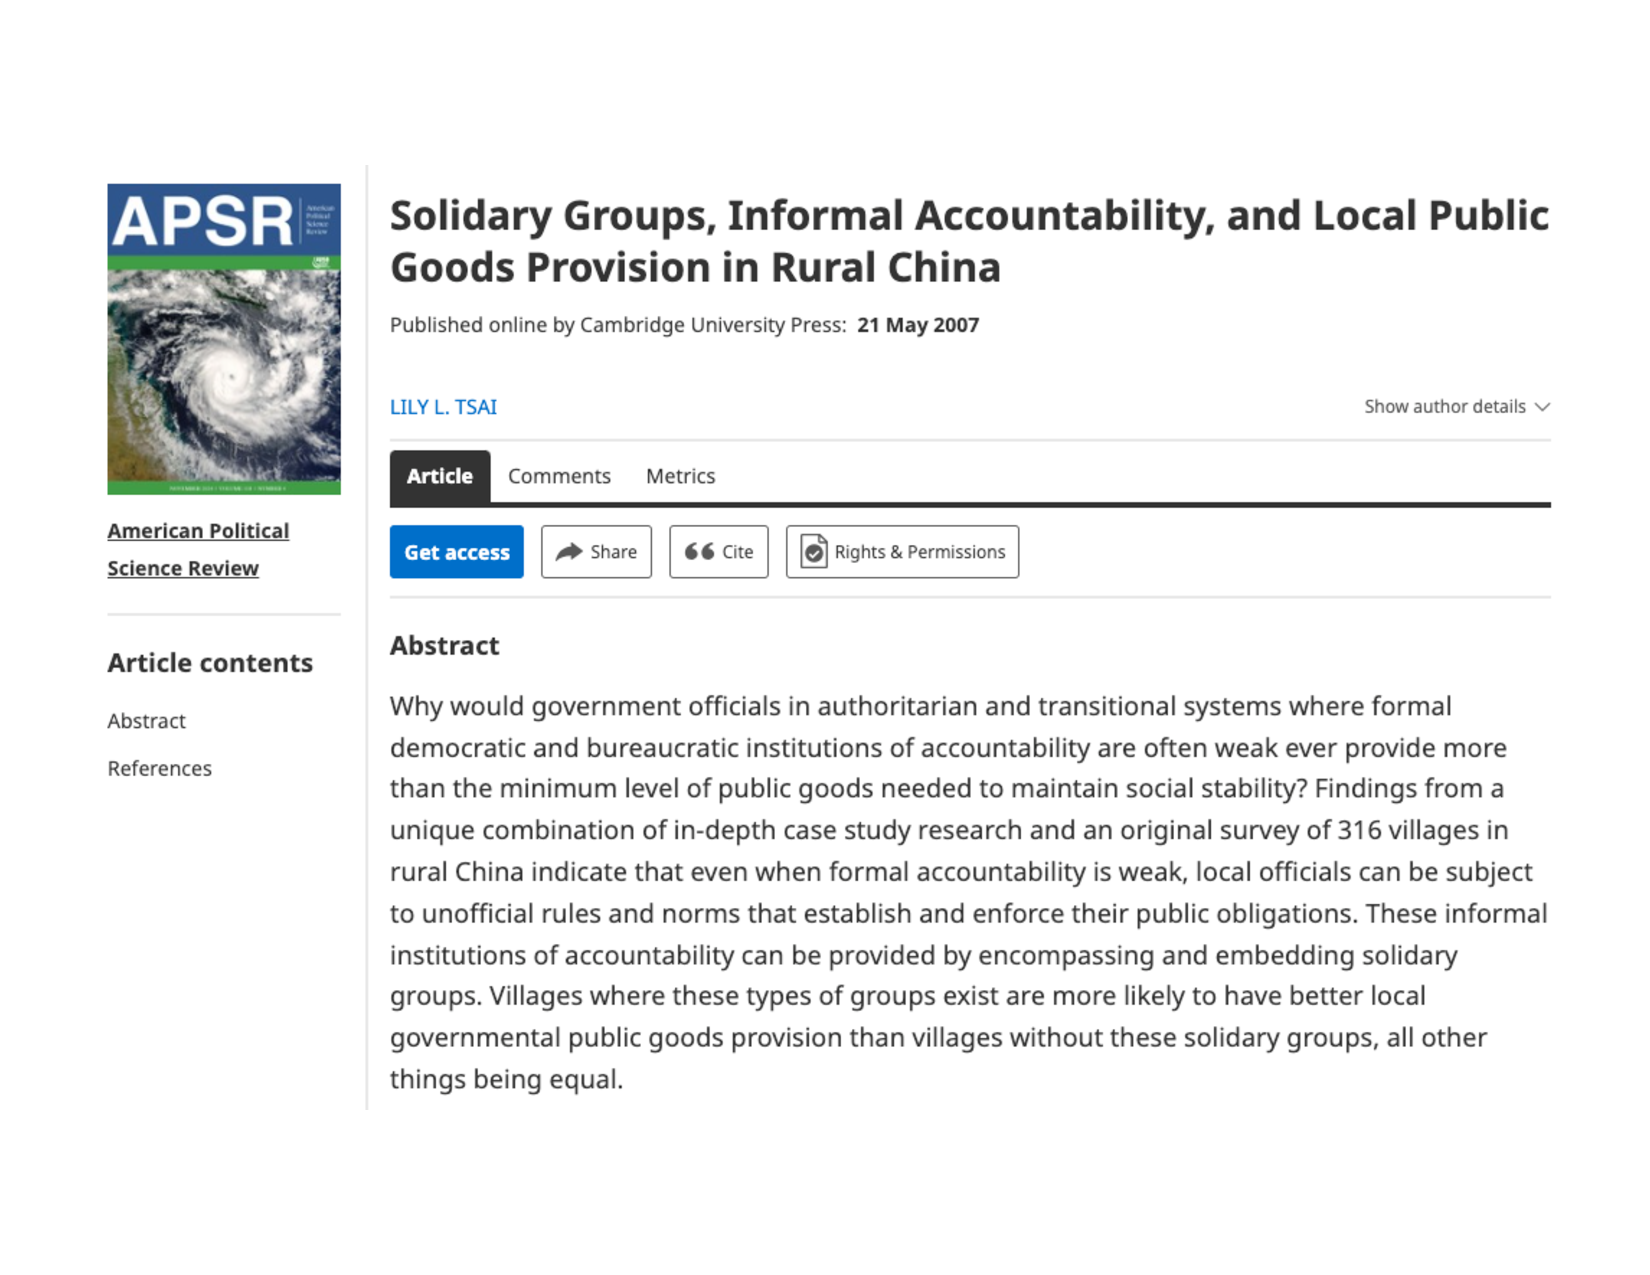
\includegraphics[width=1\linewidth]{Figs/tsai} \end{center}
\end{frame}

\begin{frame}
\begin{center}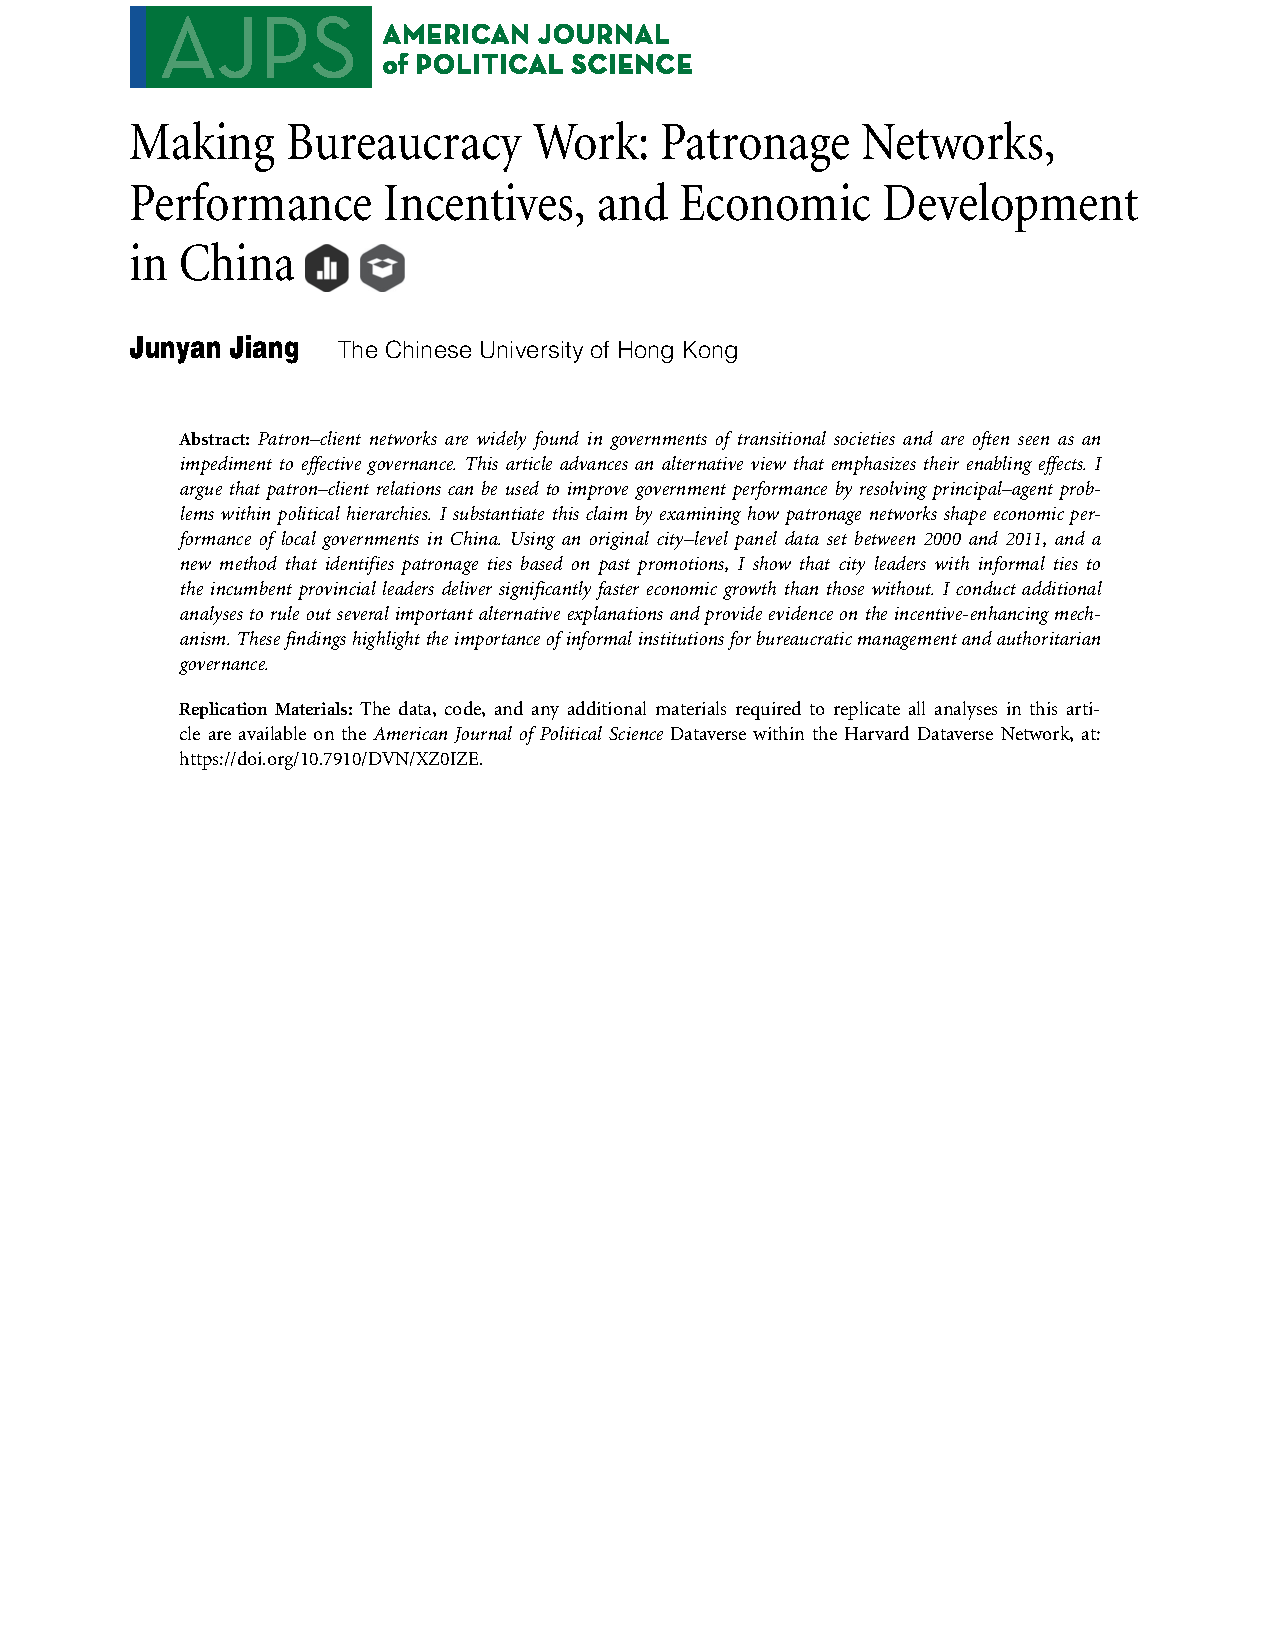
\includegraphics[width=0.95\linewidth]{Figs/jiang} \end{center}
\end{frame}

\begin{frame}
\begin{itemize}
  \item From intelligence services to academic research
  \vspace{0.3cm}
  \item From area studies to comparative politics
  \vspace{0.3cm}
  \item From qualitative description to data-intensive inference
  \vspace{0.1cm}
  \begin{itemize}
    \item Before the diplomatic reconciliation between PRC and USA (1971-1978), scholars have to rely on limited, parrial and often biased qualitative evidence (archives and interviews)
    \item After Reform and Opening, in the 1980s more engaging field research is likely (ethnography and case studies)
    \item The mid-1990s saw the quantitative turn of China studies (surveys, econometric analysis of admin data and computational)
  \end{itemize}
\end{itemize}
\end{frame}

\begin{frame}
\begin{center}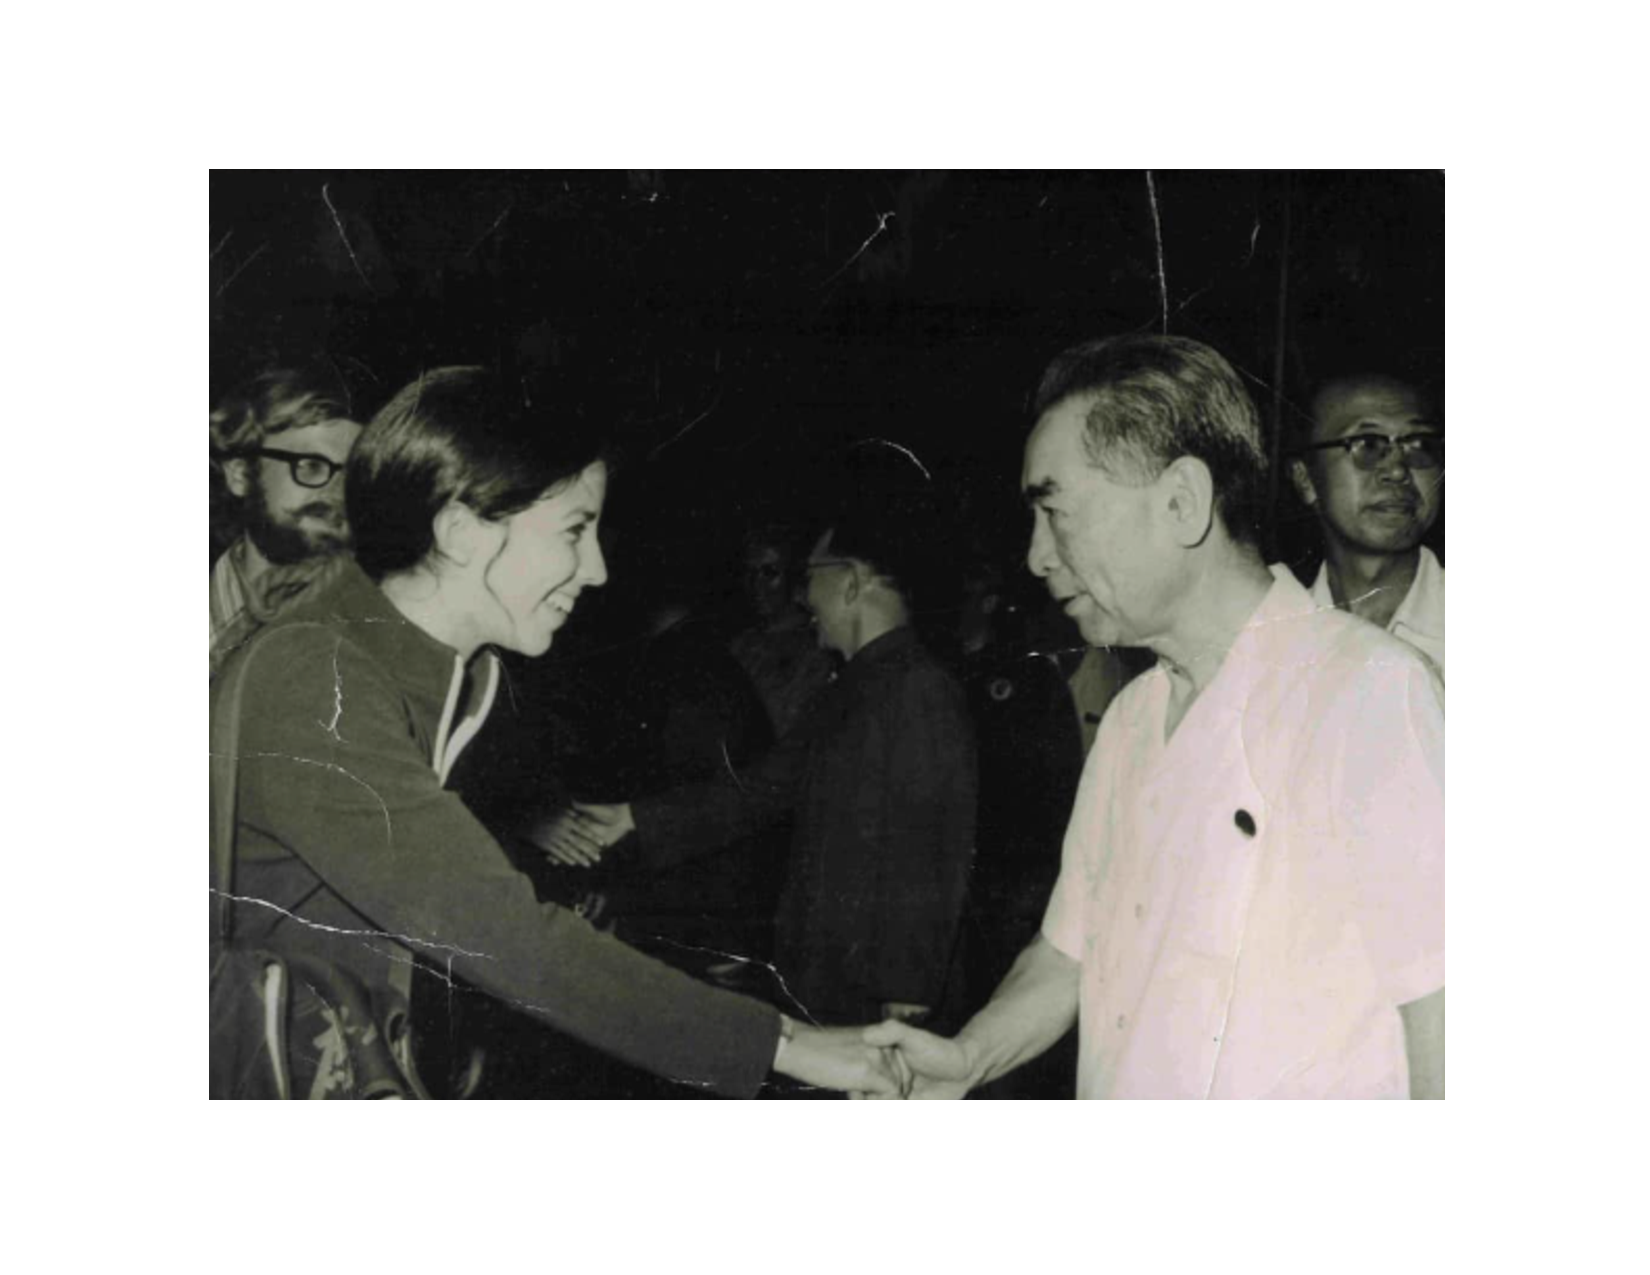
\includegraphics[width=0.9\linewidth]{Figs/shirk71} \end{center}
\vspace{0.1cm}
\begin{center}
\scriptsize
\small
Susan Shirk (UCSD) with Zhou Enlai in July 1971, on a visit to China with "the Committee of Concerned Asian Scholars"
\end{center}
\end{frame}

\begin{frame}
\begin{center}
\textbf{Week 2: Empire to Nation-State}
\end{center}
\vspace{0.3cm}

\begin{center}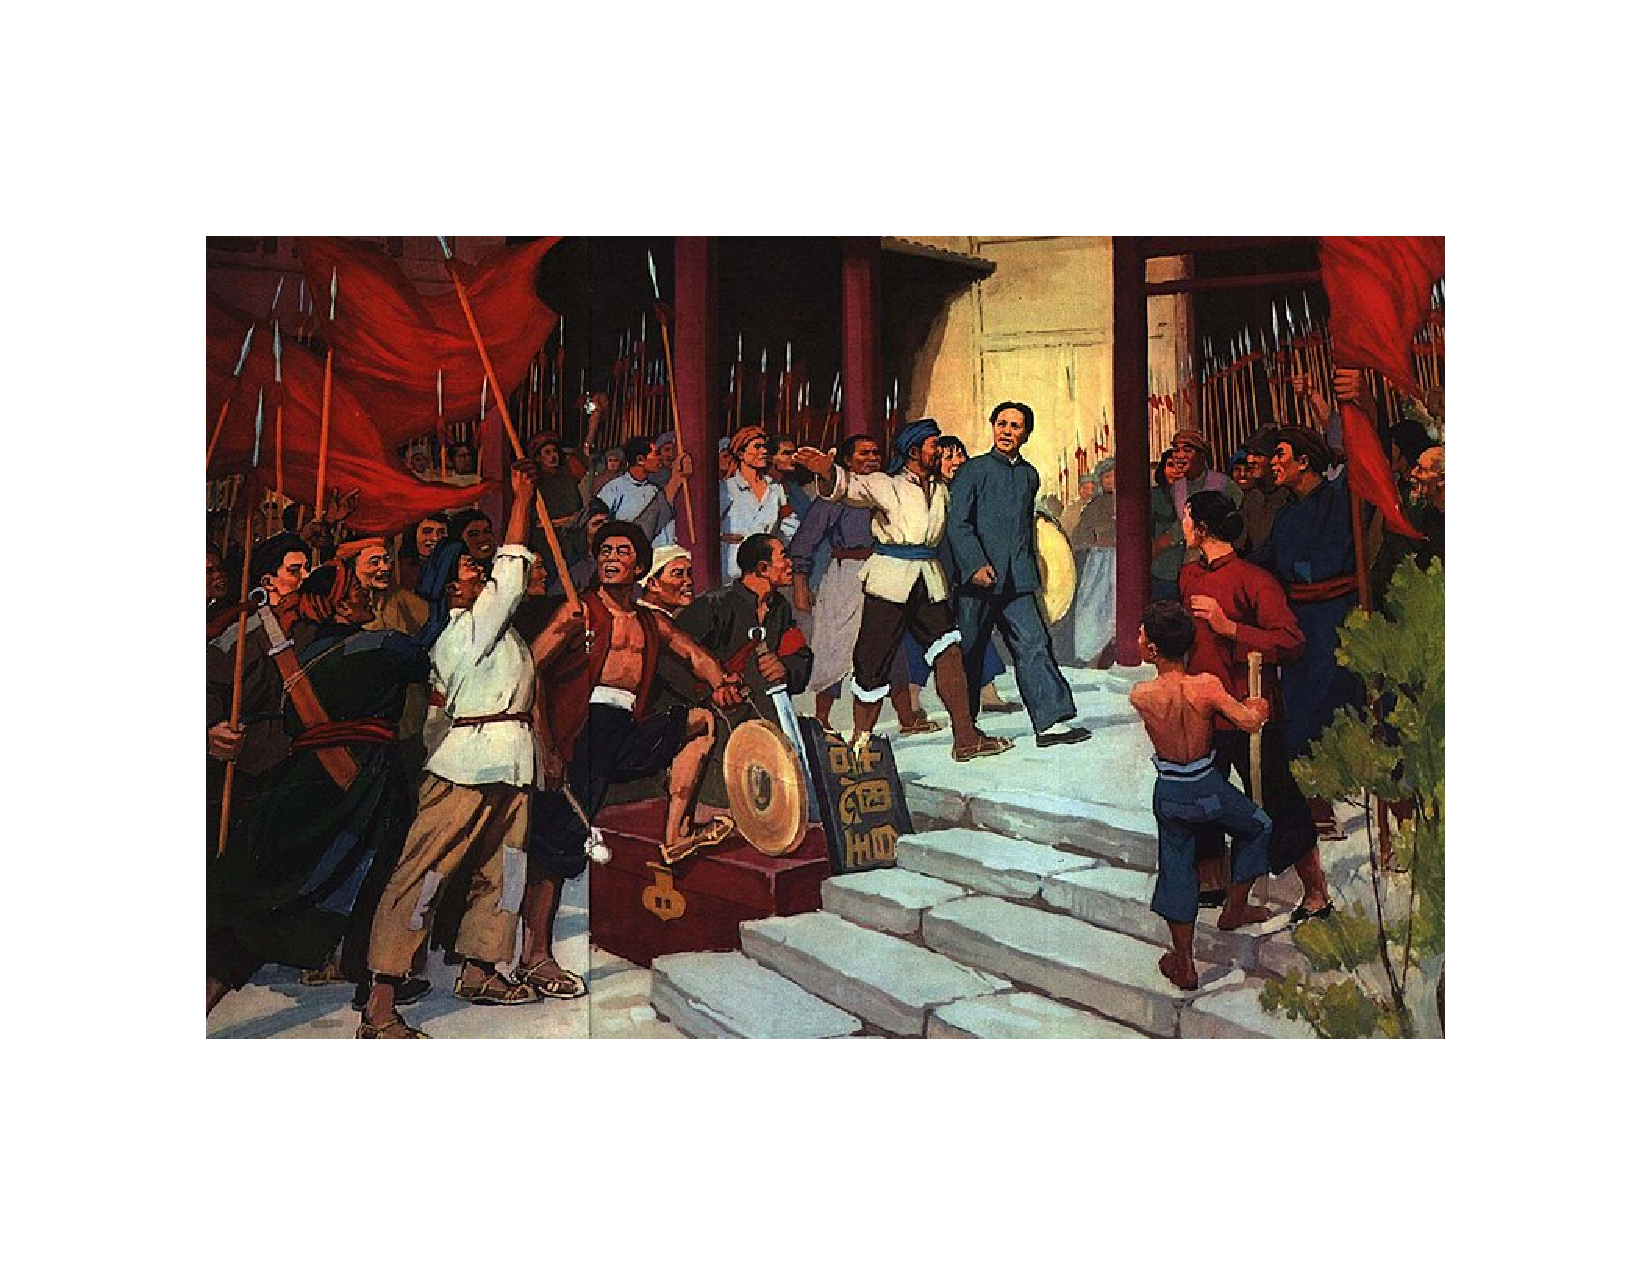
\includegraphics[width=0.7\linewidth]{Figs/theme2} \end{center}
\begin{center}
\footnotesize
\url{https://storystudio.tw/article/gushi/the-forbidden-garden}
\end{center}
\end{frame}

\begin{frame}{``China: A Century of Revolution''}
\phantomsection\label{china-a-century-of-revolution}
\begin{center}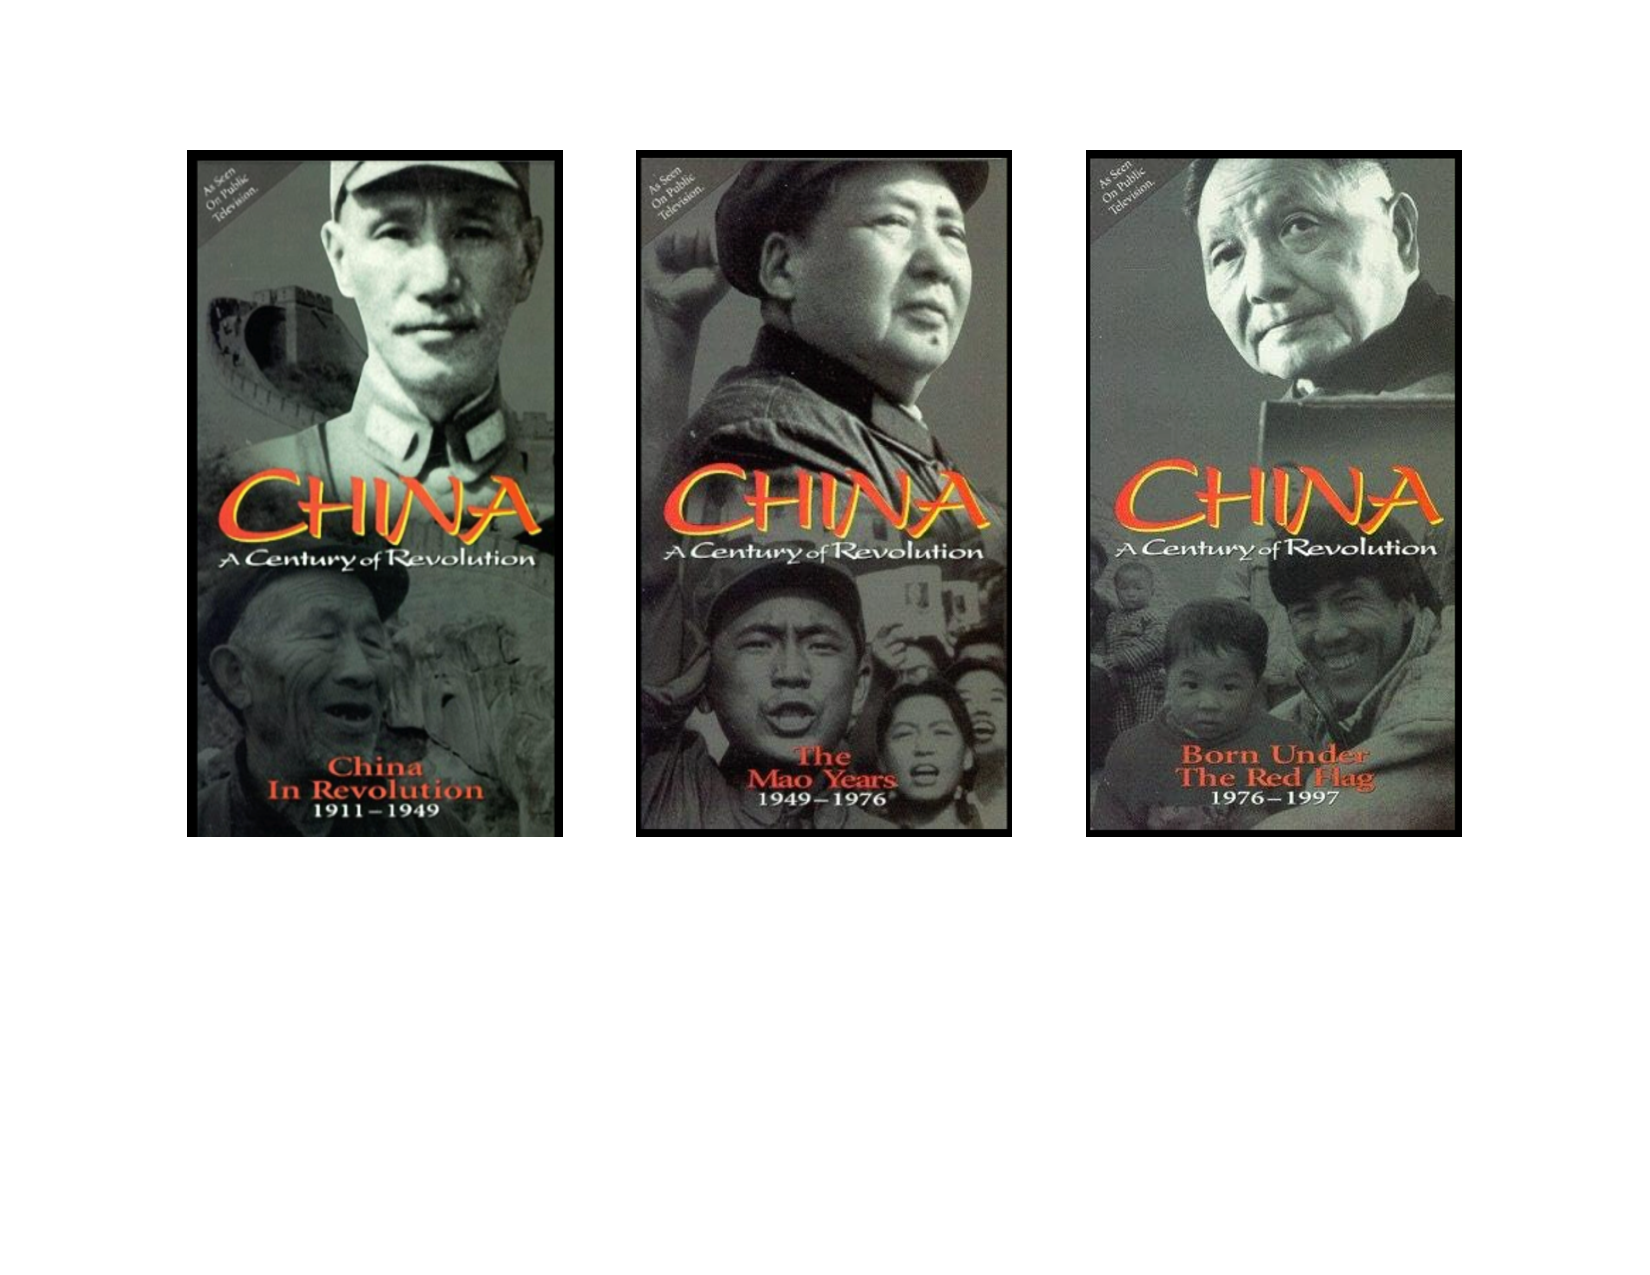
\includegraphics[width=0.95\linewidth]{Figs/docs} \end{center}
\end{frame}

\begin{frame}{China in the 20th century}
\phantomsection\label{china-in-the-20th-century}
\begin{itemize}
  \item Republican China (1911-1949)
  \vspace{0.2cm}
  \begin{itemize}
    \item 1911-1928: Beiyang Government
    \item 1928-1949: Nationalist/KMT Government 
  \end{itemize}
  \vspace{0.4cm}
  \item Communist China (1949 and afterwards)
  \vspace{0.2cm}
  \begin{itemize}
    \item 1950s: Land reform and the Great Leap Forward (大跃进)
    \item 1960s: Return of Mao Zedong and the outbreak of the Cultural Revolution (文化大革命)
    \item 1970s: Power transition and "Reform and Opening" (改革开放)
    \item 1980s: Experiment with market economy, intra-party split and Tiananmen
    \item 1990s: Consolidated market reform and institutionalized political succession
  \end{itemize}
\end{itemize}
\end{frame}

\begin{frame}{The pursuit of a ``modern'' China}
\phantomsection\label{the-pursuit-of-a-modern-china}
\begin{itemize}
  \item Question: How do we define "modernity?"
  \pause
  \vspace{0.3cm}
  \item "Modernization" is a multi-dimensional concept
  \vspace{0.1cm}
  \begin{itemize}
    \item Political modernization: Transforming the empire to a nation-state with well-established centralized state apparatus and a shared national identity
    \item Social modernization: Filling the moral vacuum with new ideas (e.g., science, democracy and vernacular language and writing) while criticizing Confucianism
    \item Economic modernization: Industrial infrastructure and production; much of this has do with security threats
  \end{itemize}
  \vspace{0.3cm}
  \item Today's discussion will focus on the first two
\end{itemize}
\end{frame}

\begin{frame}{Beiyang government in Beijing (1911-1928)}
\phantomsection\label{beiyang-government-in-beijing-1911-1928}
\begin{itemize}
  \item A weak central government that could not command
  \vspace{1cm}
  \item KMT chose to work with the Communist International in Moscow and yet faced internal power struggle
  \vspace{1cm}
  \item The "CPC-KMT" United Front collapsed and led to the first Chinese Civil War
\end{itemize}
\end{frame}

\begin{frame}
\begin{itemize}
\small
  \item A weak central government that could not command
  \vspace{0.1cm}
  \begin{itemize}
    \item \textbf{Sun Yat-sen} (孙中山) and KMT failed to control the central government in the 1911 Wuchang Uprising (武昌起义), the new ROC government was a fraigle coalition between KMT and \textbf{Yuan Shi-kai} (袁世凯, the leader of Beiyang Army)
    \item Yuan managed to become the President in 1912, but the Beiyang government in Beijing the new government remained weak, as powerful \textbf{warlords} across the country dominated in their respective jurisdictions
    \item Vibrant social movements against warlords and "Imperialism" (e.g., the May-Fourth Movement in 1919)
  \end{itemize}
  \vspace{0.4cm}
  \item KMT chose to work with the Communist International in Moscow and yet faced internal power struggle
  \vspace{0.4cm}
  \item The "CPC-KMT" United Front collapsed and led to the first Chinese Civil War
\end{itemize}
\end{frame}

\begin{frame}
\begin{itemize}
\small
  \item A weak central government that could not command
  \vspace{0.4cm}
  \item KMT chose to work with the Communist International in Moscow and yet faced internal power struggle
  \vspace{0.1cm}
  \begin{itemize}
    \item Sun sought to work with warloards in Southern China and recreated KMT with the help from the former Soviet Union in 1919
    \item With the alliance between KMT and the \textbf{Communist International}, KMT decided to form a "United Front" with the \textbf{Communist Party of China} (CPC), which was established in Shanghai, in 1921
    \item Sun passed away suddenly in 1925, and the KMT was dragged into power struggle as it was unclear who should lead
    \item \textbf{Chiang Kai-shek} managed to control the KMT and started the \textbf{Northern Expedition} (北伐) to unite the whole China in 1926
  \end{itemize}
  \vspace{0.4cm}
  \item The "CPC-KMT" United Front collapsed and led to the first Chinese Civil War
\end{itemize}
\end{frame}

\begin{frame}
\begin{itemize}
\small
  \item A weak central government that could not command
  \vspace{0.4cm}
  \item KMT chose to work with the Communist International in Moscow and yet faced internal power struggle
  \vspace{0.4cm}
  \item The "CPC-KMT" United Front collapsed and led to the first Chinese Civil War
  \vspace{0.1cm}
  \begin{itemize}
    \item As the KMT inner-circle became fragmented and divided between Chiang and others, CPC became the target of political purges
    \item The exact reason and process remain somewhat debated, but in 1927 Chiang launched the \textbf{"412 Incident"} in Shanghai -- many CPC members were arrested and executed
    \item The CPC was forced to rebuilt their power base in the countryside, adopted guerrilla warfare, and formed the first Chinese Soviet government in {Jiangxi}
    \item Chiang managed to control the entire China in 1928, at least nominally, and set the capital in {Nanjing}
  \end{itemize}
\end{itemize}
\end{frame}

\begin{frame}{Nationalist government in Nanjing (1928-1949)}
\phantomsection\label{nationalist-government-in-nanjing-1928-1949}
\begin{itemize}
  \item State building and socio-economic rebuilding
  \vspace{1cm}
  \item First Chinese Civil War and the rise of Mao within CPC
  \vspace{1cm}
  \item Anti-Japanese War and Chiang's downfall in 1949
\end{itemize}
\end{frame}

\begin{frame}
\begin{itemize}
  \item State building and socio-economic rebuilding
  \vspace{0.1cm}
  \begin{itemize}
    \item The decade before 1937 was often known as the \textbf{Nanjing Decade} or \textbf{Golden Decade}, during which China saw remarkable economic and market growth (and industrialization)
    \item The KMT govt under Chiang introduced the new Life Movement while strenthening the system of taxation and civil services through the Examination Yuan and the self-government movement
    \item See \textit{Strong Institutions and Weak Polities} by Julia Strauss (SOAS)
  \end{itemize}
  \vspace{0.6cm}
  \item First Chinese Civil War (1927-1936) and the rise of Mao within CPC
  \vspace{0.6cm}
  \item Anti-Japanese War and Chiang's downfall in 1949
\end{itemize}
\end{frame}

\begin{frame}
\begin{itemize}
  \item State building and socioeconomic recovery
  \vspace{0.6cm}
  \item First Chinese Civil War (1927-1936) and the rise of Mao within CPC
  \vspace{0.1cm}
  \begin{itemize}
    \item The fallout of the first United Front in 1927 forced the CPC to "flee" to the countryside and triggered an internal debate
    \item During the \textbf{Long March} (长征), Mao managed to gain the leadership within the Party and was able to start a series of political movements to secure his power once the Party reached Yan'an
    \item The Xi'an Incident (西安事变) in 1936 forced him to declare another "CPC-KMT" United Front
    \item During the Anti-Japnese War, the CPC continued to grow its base, largely in Northern parts of the country 
  \end{itemize}
  \vspace{0.6cm}
  \item Anti-Japanese War and Chiang's downfall in 1949
\end{itemize}
\end{frame}

\begin{frame}
\begin{itemize}
  \item State building and socioeconomic recovery
  \vspace{0.6cm}
  \item First Chinese Civil War (1927-1936) and the rise of Mao within CPC
  \vspace{0.6cm}
  \item Anti-Japanese War and Chiang's downfall in 1949
  \vspace{0.1cm}
  \begin{itemize}
    \item The conflict between CPC and KMT was resumed quickly after the WWII ended in 1945
    \item The Chongqing Negotiations (with the involvement of the US) between Mao and Chiang failed 
    \item CPC won the Second Chinese Civil War (1946-1950) and established the PRC while Chiang relocated the KMT government to Taiwan in 1949
  \end{itemize}
\end{itemize}
\end{frame}

\begin{frame}{Nationalist government in Nanjing (1928-1949)}
\phantomsection\label{nationalist-government-in-nanjing-1928-1949-1}
\begin{itemize}
  \item State building and socio-economic rebuilding
  \vspace{1cm}
  \item First Chinese Civil War and the rise of Mao within CPC
  \vspace{1cm}
  \item Anti-Japanese War and Chiang's downfall in 1949
\end{itemize}
\end{frame}

\begin{frame}
\begin{itemize}
  \item State building and socio-economic rebuilding
  \vspace{0.1cm}
  \begin{itemize}
    \item The decade before 1937 was often known as the \textbf{Nanjing Decade} or \textbf{Golden Decade}, during which China saw remarkable economic and market growth (and industrialization)
    \item The KMT govt under Chiang introduced the new Life Movement while strenthening the system of taxation and civil services through the Examination Yuan and the self-government movement
    \item See \textit{Strong Institutions and Weak Polities} by Julia Strauss (SOAS)
  \end{itemize}
  \vspace{0.6cm}
  \item First Chinese Civil War (1927-1936) and the rise of Mao within CPC
  \vspace{0.6cm}
  \item Anti-Japanese War and Chiang's downfall in 1949
\end{itemize}
\end{frame}

\begin{frame}
\begin{itemize}
  \item State building and socio-economic rebuilding
  \vspace{0.6cm}
  \item First Chinese Civil War (1927-1936) and the rise of Mao within CPC
  \vspace{0.1cm}
  \begin{itemize}
    \item The fallout of the first United Front in 1927 forced the CPC to "flee" to the countryside and triggered an internal debate
    \item During the \textbf{Long March} (长征), Mao managed to gain the leadership within the Party in the Zunyi Conference (遵义会议) and mobilized a series of political movements to secure his power once the Party reached Yan'an
    \item The Xi'an Incident (西安事变) in 1936 forced him to declare another "CPC-KMT" United Front
    \item During the Anti-Japnese War, the CPC continued to grow its base, largely in Northern parts of the country 
  \end{itemize}
  \vspace{0.6cm}
  \item Anti-Japanese War and Chiang's downfall in 1949
\end{itemize}
\end{frame}

\begin{frame}
\begin{itemize}
  \item State building and socio-economic rebuilding
  \vspace{0.6cm}
  \item First Chinese Civil War (1927-1936) and the rise of Mao within CPC
  \vspace{0.6cm}
  \item Anti-Japanese War and Chiang's downfall in 1949
  \vspace{0.1cm}
  \begin{itemize}
    \item The conflict between CPC and KMT was resumed quickly after the WWII ended in 1945
    \item The Chongqing Negotiations (with the involvement of the US) between Mao and Chiang failed 
    \item CPC won the Second Chinese Civil War (1946-1950) and established the PRC while Chiang relocated the KMT government to Taiwan in 1949
  \end{itemize}
\end{itemize}
\end{frame}

\begin{frame}
\vspace{0.3cm}

\begin{center}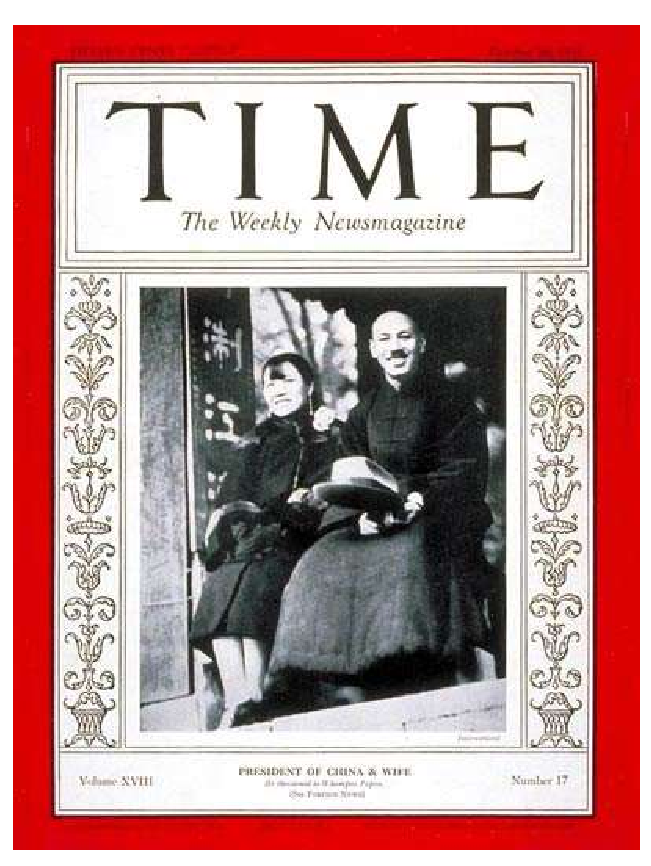
\includegraphics[width=0.5\linewidth]{Figs/chiang_new} \end{center}
\end{frame}

\begin{frame}
\vspace{0.3cm}

\begin{center}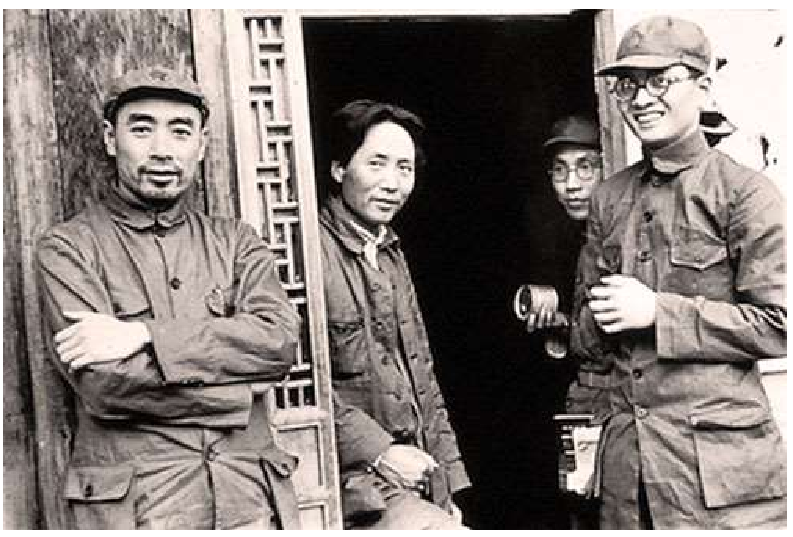
\includegraphics[width=0.9\linewidth]{Figs/yanan_new} \end{center}
\end{frame}

\begin{frame}
\vspace{0.3cm}

\begin{center}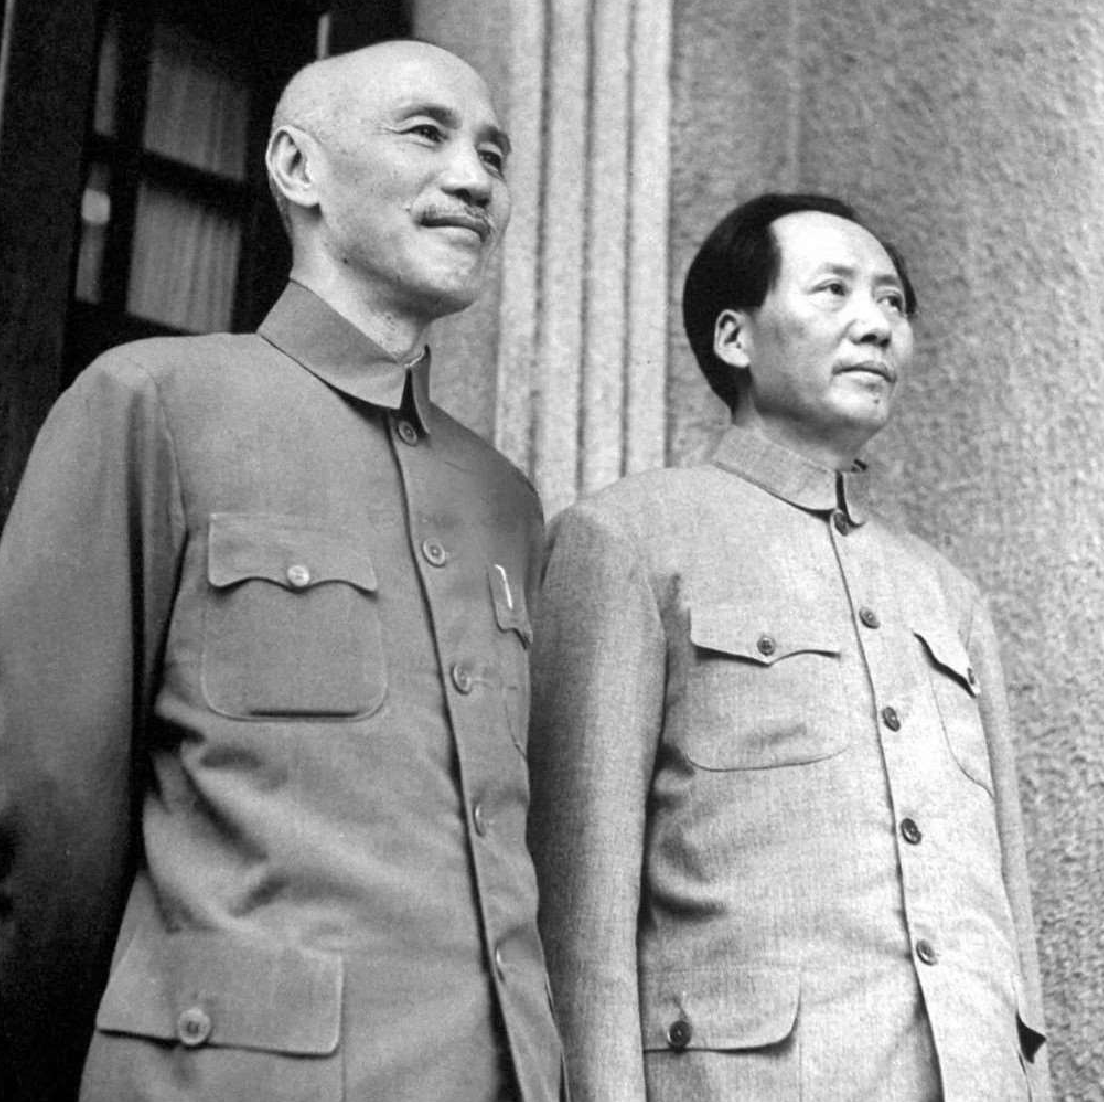
\includegraphics[width=0.6\linewidth]{Figs/chongqing_new} \end{center}
\end{frame}

\begin{frame}{Questions remain for China and comparative scholars}
\phantomsection\label{questions-remain-for-china-and-comparative-scholars}
\begin{itemize}
\small
  \item For China scholars
  \vpsace{0.1cm}
  \begin{itemize}
    \item What explains CPC's victory? Is it "predictable" or "expected?" Lieberthal (1995): The GMD's defeat was the result of its separation from its political and economic base
    \item Much of te long-term impact of the Chinese revolutions remains to be explored (e.g., Elizabeth Perry)
    \item Information needed to study the early 20th century of China is all over the place, and many informants may no longer be around
  \end{itemize}
  \vpsace{0.3cm}
  \item Chinese revolution(s) in comparative perspective
  \vpsace{0.1cm}
  \begin{itemize}
    \item Causes, results and implications for long-term political development (Moore 1966; Skocpol 1979; Way and Levitsky 2022)
    \item Political elites and leadership "style" (e.g., compared with the former Soviet Union)
    \item Revolutionary party v ruling party (Lee 1990; Harding 1981)
  \end{itemize}  
\end{itemize}
\end{frame}

\begin{frame}
Perry
\end{frame}

\begin{frame}
Ma and Ji
\end{frame}

\begin{frame}
Lee
\end{frame}

\begin{frame}
Moore; Skocpol; Way and Levitsky
\end{frame}

\begin{frame}{Local states in the early 20th century (Remick 2002)}
\phantomsection\label{local-states-in-the-early-20th-century-remick-2002}
\begin{itemize}
  \item Key idea(s): The behavior and capacity of local states vary significantly in China, as these two are shaped by central policy and local social contexts (history, limitations and ideology)
  \vspace{0.3cm}
  \item Some questions to consider:
  \vspace{0.1cm}
  \begin{itemize}
    \item What is a state and state "capacity?" How did Remick define it? Why is state-building an important question? Why did she and many scholars choose to focus on taxation and public finance?
    \item Why do we need to look central and local state-building as two distinctive and yet interrelated processes?
    \item She mentioned a couple of countries to put her argument in a comparative perspective. Why? Does it make sense to you? Any other cases you can think of?
  \end{itemize}
\end{itemize}
\end{frame}

\begin{frame}
\vspace{1cm}

See you next week!
\end{frame}

\begin{frame}{Appendix: Key events during the Republican Era}
\phantomsection\label{appendix-key-events-during-the-republican-era}
\begin{itemize}
  \item Beiyang period
  \vspace{0.1cm}
  \begin{itemize}
    \item 1919: May-Fourth Movement (五四运动) and the recreation of new KMT
    \item 1926-1928: North Expedition (北伐)
  \end{itemize}
  \vspace{0.3cm}
  \item Republican period
  \begin{itemize}
    \item 1927-1936: 1st CPC-KMT Civil War (一次国共内战)
    \item 1934-1935: Long March (长征) and Zunyi Conference (遵义会议)
    \item 1937-1945: Anti-Japanese War (抗日战争)
    \item 1942-1945: Rectification Movement (整风运动)
    \item 1945-1949: 2nd CPC-KMT Civil War (二次国共内战)
  \end{itemize}
\end{itemize}
\end{frame}

\begin{frame}{Appendix: CPC v KMT}
\phantomsection\label{appendix-cpc-v-kmt}
\begin{itemize}
  \item KMT: Started as a revolutionary party rallying around Sun Ya-sen, and yet fraught with corruption and internal fragmentation
  \vspace{1cm}
  \item CPC: Started as an urban party with the (selective) support from the Communist International; relationship with GMD falling out and had to change and survive
\end{itemize}
\end{frame}

\end{document}
